%        File: DesignDocument.tex
%     Created: 一 3月 26 01:00 下午 2018 C
% Last Change: 一 3月 26 01:00 下午 2018 C
%
\documentclass[UTF8,noindent]{ctexart}
\usepackage[a4paper,left=2.0cm,right=2.0cm,top=2.0cm,bottom=2.0cm]{geometry}
\usepackage{hyperref}
\usepackage{url}
\usepackage{graphicx}
\usepackage{amsmath}
\usepackage{amssymb}
\usepackage{enumitem}
\usepackage{tikz}
\usepackage{float}
\usepackage{xeCJK}
\usepackage{listings}
\usepackage{xcolor}
\lstset{language = c,numbers=left, showstringspaces=false,keywordstyle= \color{ blue!70 },commentstyle=\color{red!50!green!50!blue!50}, frame=shadowbox, rulesepcolor= \color{ red!20!green!20!blue!20 } 
} 
\usetikzlibrary{graphs}
\title{\CJKfamily{zhkai}计算机网络研讨课实验报告}
\author{{\CJKfamily{zhkai}冯吕}\ $2015K8009929049$}
\date{\today}
\begin{document}
\maketitle
\zihao{5}
\CJKfamily{zhsong}
\begin{center}
  \begin{tabular}{|p{15cm}|}
	\hline
	{\CJKfamily{zhhei}实验题目}:$Socket$ 应用编程实验\\
	\hline 
	{\CJKfamily{zhhei}实验内容}:在本次实验中,需要实现一个基于$Socket$的字符统计程序。首先,有两个文件,$workers.conf$配置文件中存储了所有$worker$的$IP$,$war_and_peace.txt$文件则是需要统计字符的文件。因此,在本次实验中,需要分别实现$master$和$worker$,首先,$master$需要读取$worker$的配置文件,即获得$worker$的$IP$,然后与$worker$建立连接,连接成功之后,将任务分发给各个$worker$,$worker$接收到消息后,进行字符统计,然后把统计结果返回给$master$,然后$master$整合统计结果并将结果输出到屏幕上。\\
	\hline
	{\CJKfamily{zhhei}实验流程}:\begin{enumerate}
	  \item $master$读取配置文件,获取$IP$,$IP$数为$2$,因此,建立两个$Socket$,分别与一个$worker$建立连接。
		\item 对于每个$worker$来说,首先创建一个$Socket$,然后进行绑定,绑定完成之后,等待着$master$来连接。
		  \item $master$与两个$worker$建立连接之后,需要分发任务。首先,通过文件操作获取文件中的总字符数目,然后将前一半分给第一个$worker$统计,后一半分给另一个。因此,发送给$worker$的消息总共占$30$个字节,四个字节为字节数,四个字节为$worker$需要统计的起始位置,四个字节为终止位置,剩余的十八个字节为文件名(包括字符串中的最后一个空字符)。
			\item 每个$worker$接收到$master$传过来的消息之后,就获取到了文件名,然后打开文件,通过$fseek$函数定位到起始位置,进行字符统计,统计所有的字母,不区分大小写。统计完成之后,再将统计结果发送回去给$master$,每个字母的数目用一个$int$型四字节存储,因此,返回给$master$的消息长度为$104$字节。
			  \item $master$收到两个$worker$返回的消息之后,将两个$worker$对应的统计值相加,然后在屏幕上输出$26$个字母的数目统计值。
	\end{enumerate}\\
	\hline
	{\CJKfamily{zhhei}实验结果}:运行截图见下页的图片,$master$与$worker$成功建立了连接,最终输出了正确统计结果。\\
	\hline
	{\CJKfamily{zhhei}结果分析}:在刚开始,由于一些内存错误,导致$worker$运行时出现$segmentation\ fault$,后经过调试,程序能够按照实验要求正确运行,输出结果与$reference$程序一样。\\
	\hline
  \end{tabular}
\end{center}
\begin{figure}[H]
  \centering
  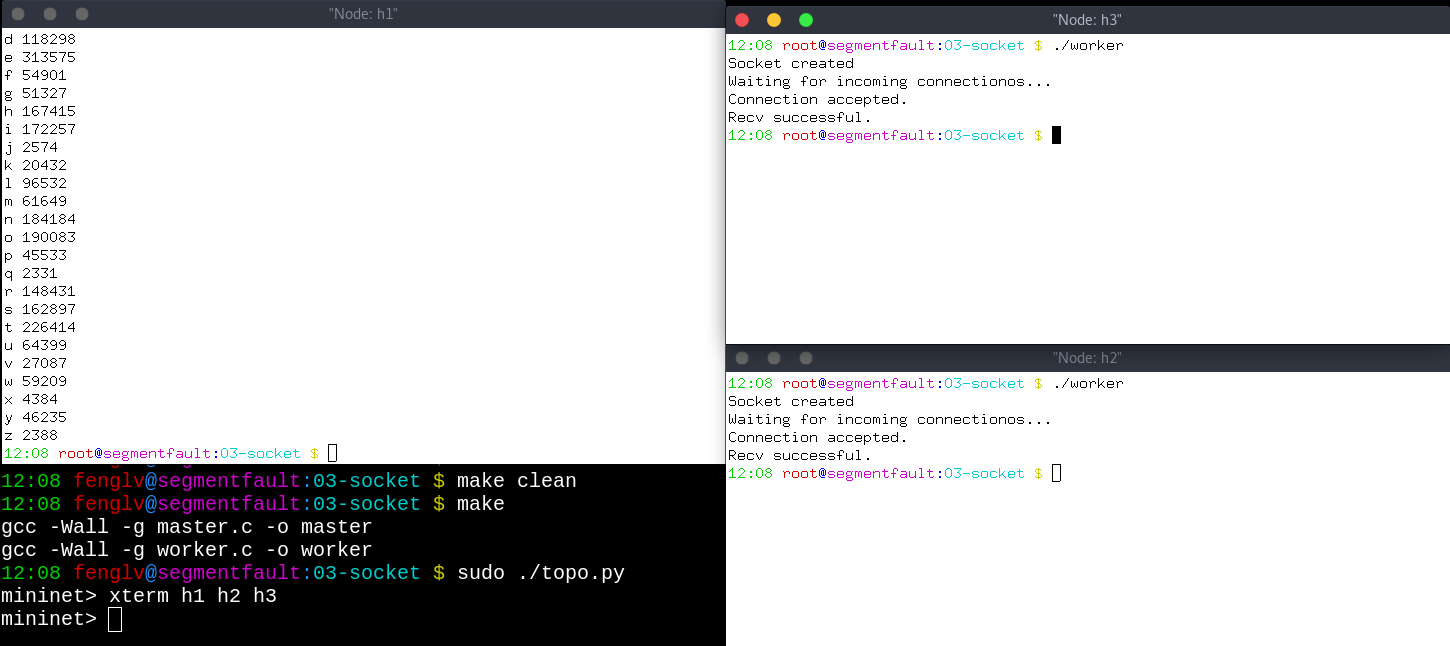
\includegraphics[scale = 0.3]{./sshot.png}
  \caption{$Socket$应用编程实验运行截图}
\end{figure}
\end{document}


